\documentclass[11pt,a4paper]{article}

% Packages for formatting and graphics
\usepackage[utf8]{inputenc}
\usepackage{geometry}
\usepackage{graphicx}
\usepackage{listings}
\usepackage{xcolor}

% Page geometry
\geometry{margin=2.5cm}

% R code styling
\definecolor{codegreen}{rgb}{0,0.6,0}
\definecolor{codegray}{rgb}{0.5,0.5,0.5}
\definecolor{codepurple}{rgb}{0.58,0,0.82}
\definecolor{backcolour}{rgb}{0.95,0.95,0.92}

\lstdefinestyle{rstyle}{
    backgroundcolor=\color{backcolour},   
    commentstyle=\color{codegreen},
    keywordstyle=\color{magenta},
    numberstyle=\tiny\color{codegray},
    stringstyle=\color{codepurple},
    basicstyle=\ttfamily\footnotesize,
    breakatwhitespace=false,         
    breaklines=true,                 
    captionpos=b,                    
    keepspaces=true,                 
    numbers=none,                    
    showspaces=false,                
    showstringspaces=false,
    showtabs=false,                  
    tabsize=2,
    frame=single,
    rulecolor=\color{blue!30!black}
}

\lstset{style=rstyle}

\begin{document}

\begin{lstlisting}[language=R]
# Load required libraries
library(ggplot2)
library(dplyr)
library(lubridate)
library(readr)

# Set working directory and read data
setwd("/home/alcafache/Documentos/PE/Exercicio3")
dados_clima <- read_csv("clima.csv", show_col_types = FALSE) %>%
  rename(datetime = Data, PRES = Pressao) %>%
  filter(year(datetime) == 2014, month(datetime) == 11) %>%
  group_by(date = as.Date(datetime)) %>%
  mutate(mediana_pressao_diaria = median(PRES, na.rm = TRUE)) %>%
  ungroup()

# Create and save plot
plot <- ggplot(dados_clima, aes(x = datetime)) +
  geom_line(aes(y = PRES, color = "Pressao Horaria"), alpha = 0.7) +
  geom_line(aes(y = mediana_pressao_diaria, color = "Mediana Diaria"), linewidth = 1) +
  labs(title = "Variacao da Pressao Atmosferica em Novembro de 2014",
       x = "Data e Hora", y = "Pressao (hPa)", color = "Legenda") +
  scale_x_datetime(date_breaks = "3 days", date_labels = "%d/%m") +
  scale_color_manual(values = c("Pressao Horaria" = "deepskyblue", "Mediana Diaria" = "red4")) +
  theme_minimal() +
  theme(axis.text.x = element_text(angle = 45, hjust = 1), legend.position = "top")

print(plot)
ggsave("clima_pressao_nov2014.png", width = 11, height = 6.5, dpi = 300)
\end{lstlisting}

\begin{figure}[htbp]
    \centering
    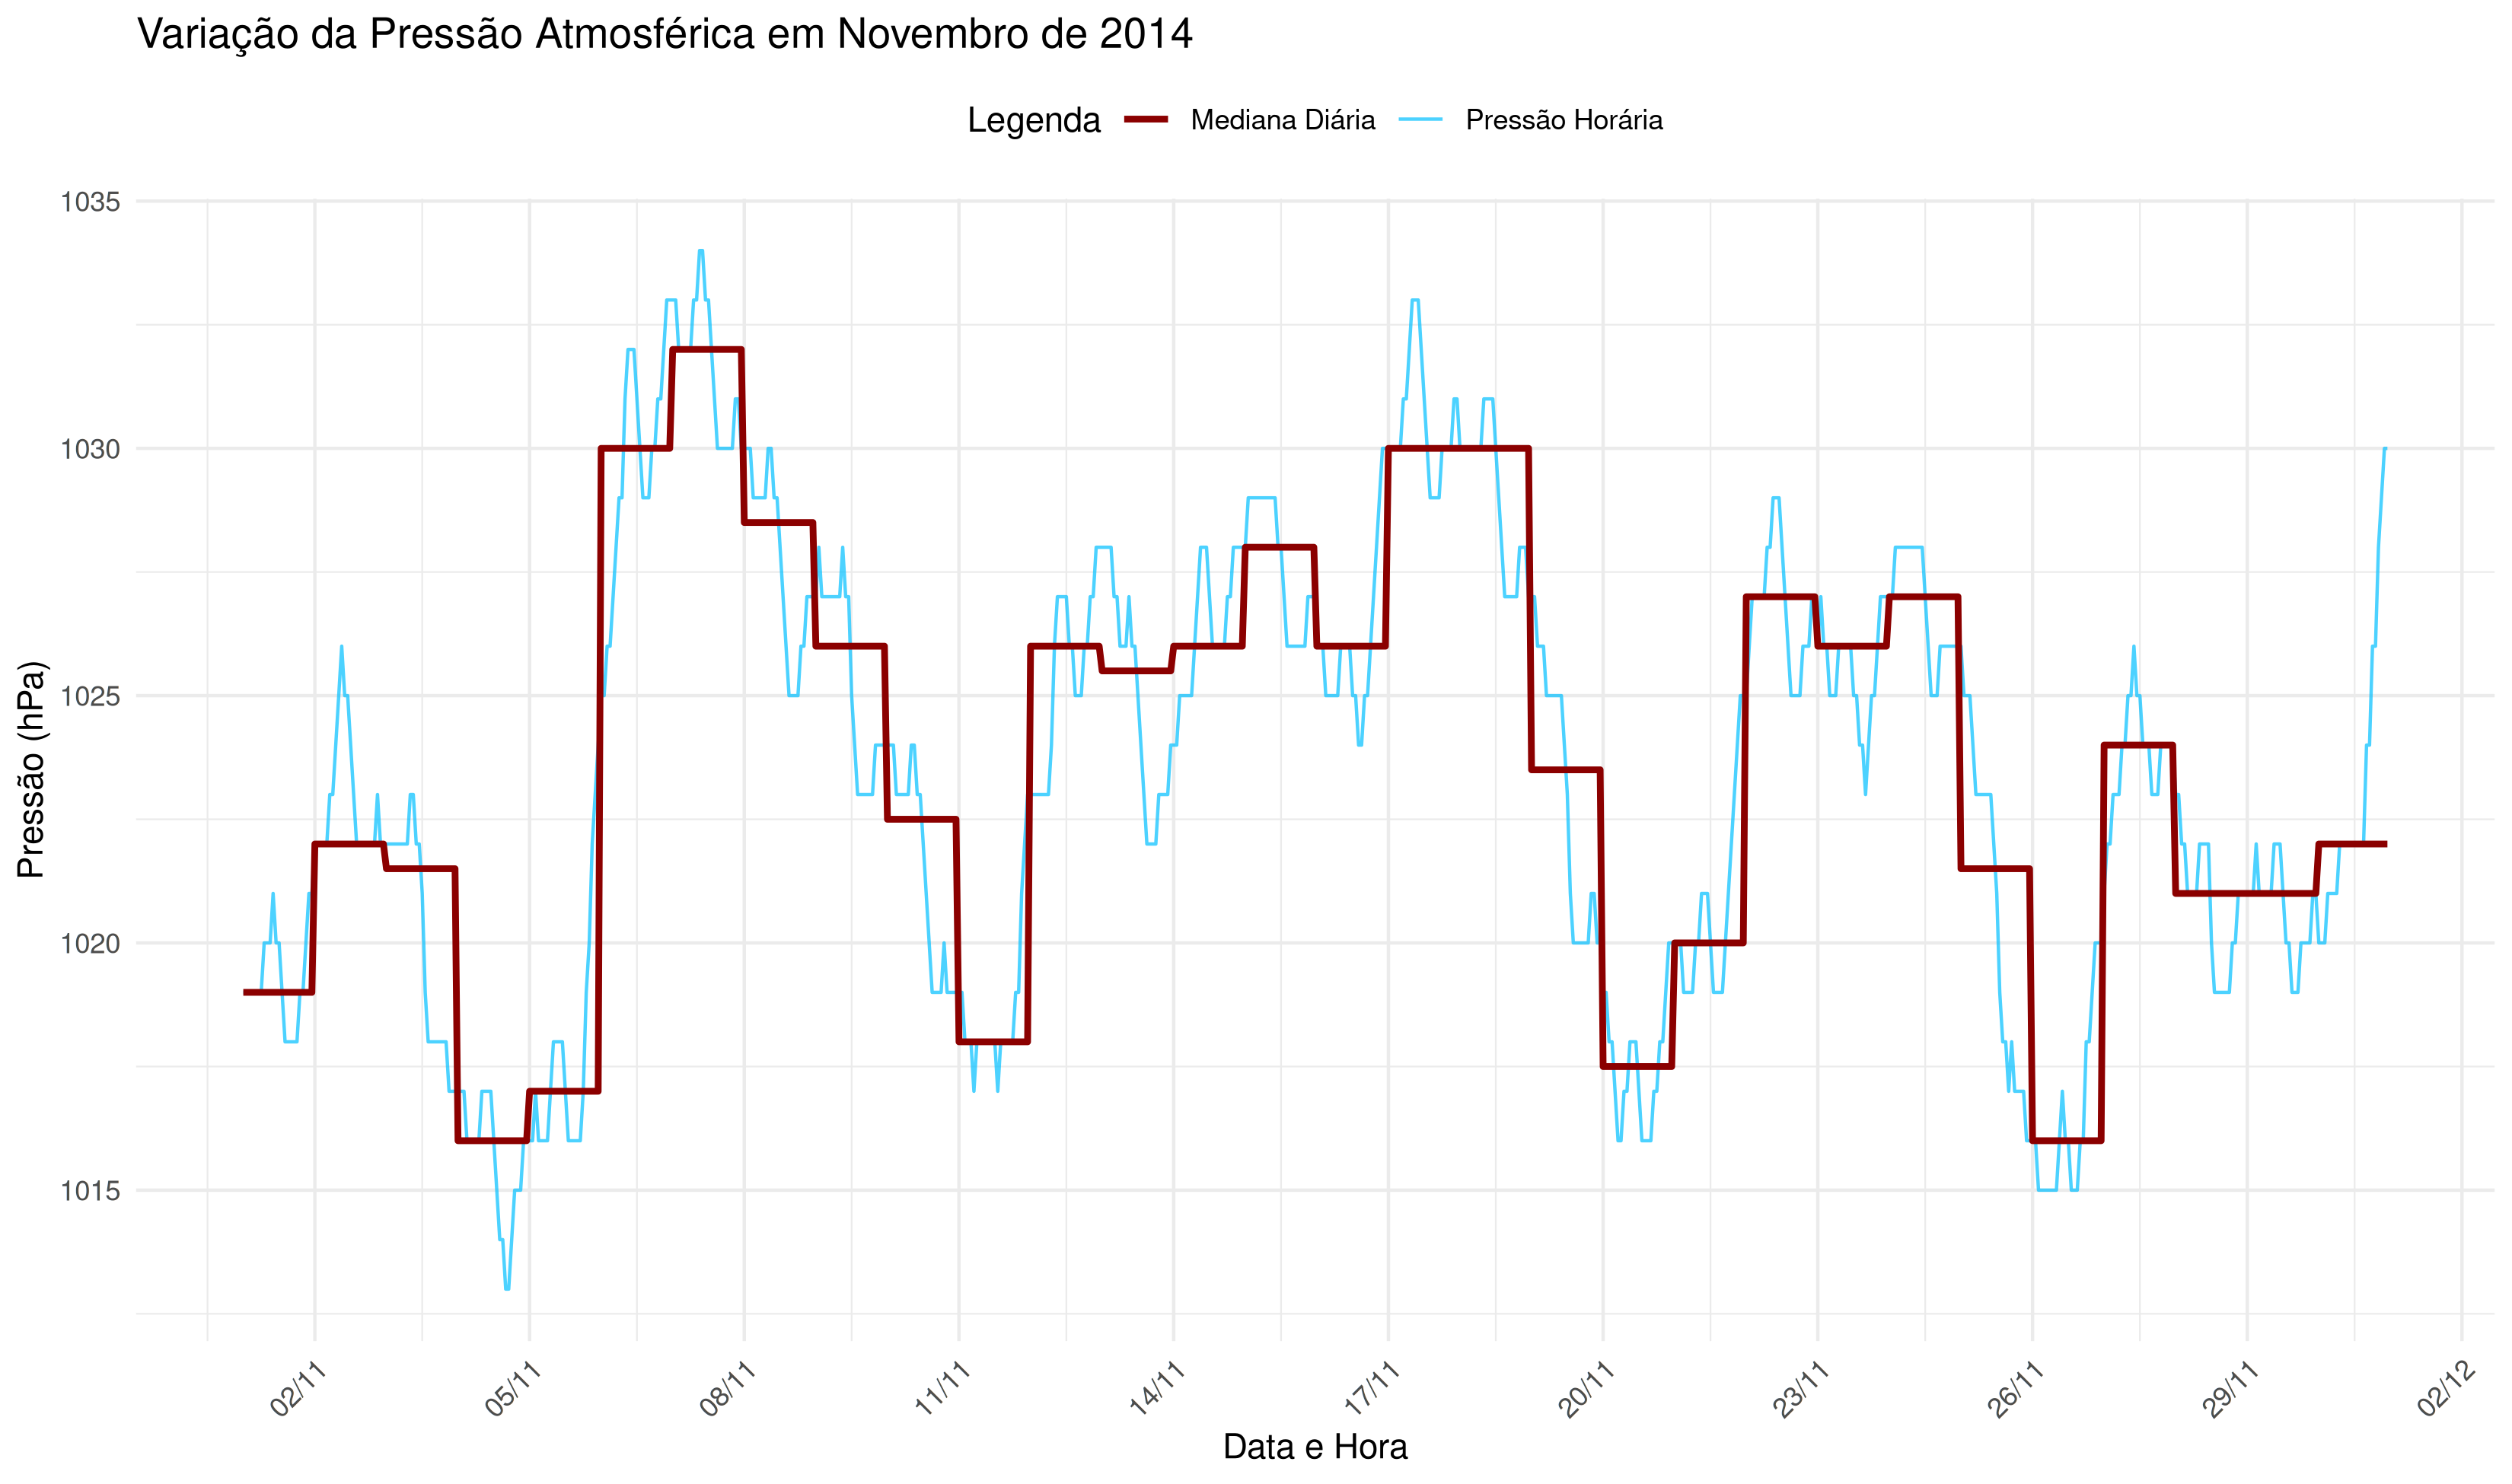
\includegraphics[width=0.9\textwidth]{clima_pressao_nov2014.png}
\end{figure}

\end{document}
